% Optional inclusion only. This file has not been inserted into the manuscript.
% Paths assume compilation from paper/acl-2027/official-template/.
% graphicx is sufficient for the 300 dpi PNG versions below.
% The source SVGs remain editable; no PDF conversion is required for this study.
\begin{figure*}[t]
  \centering
  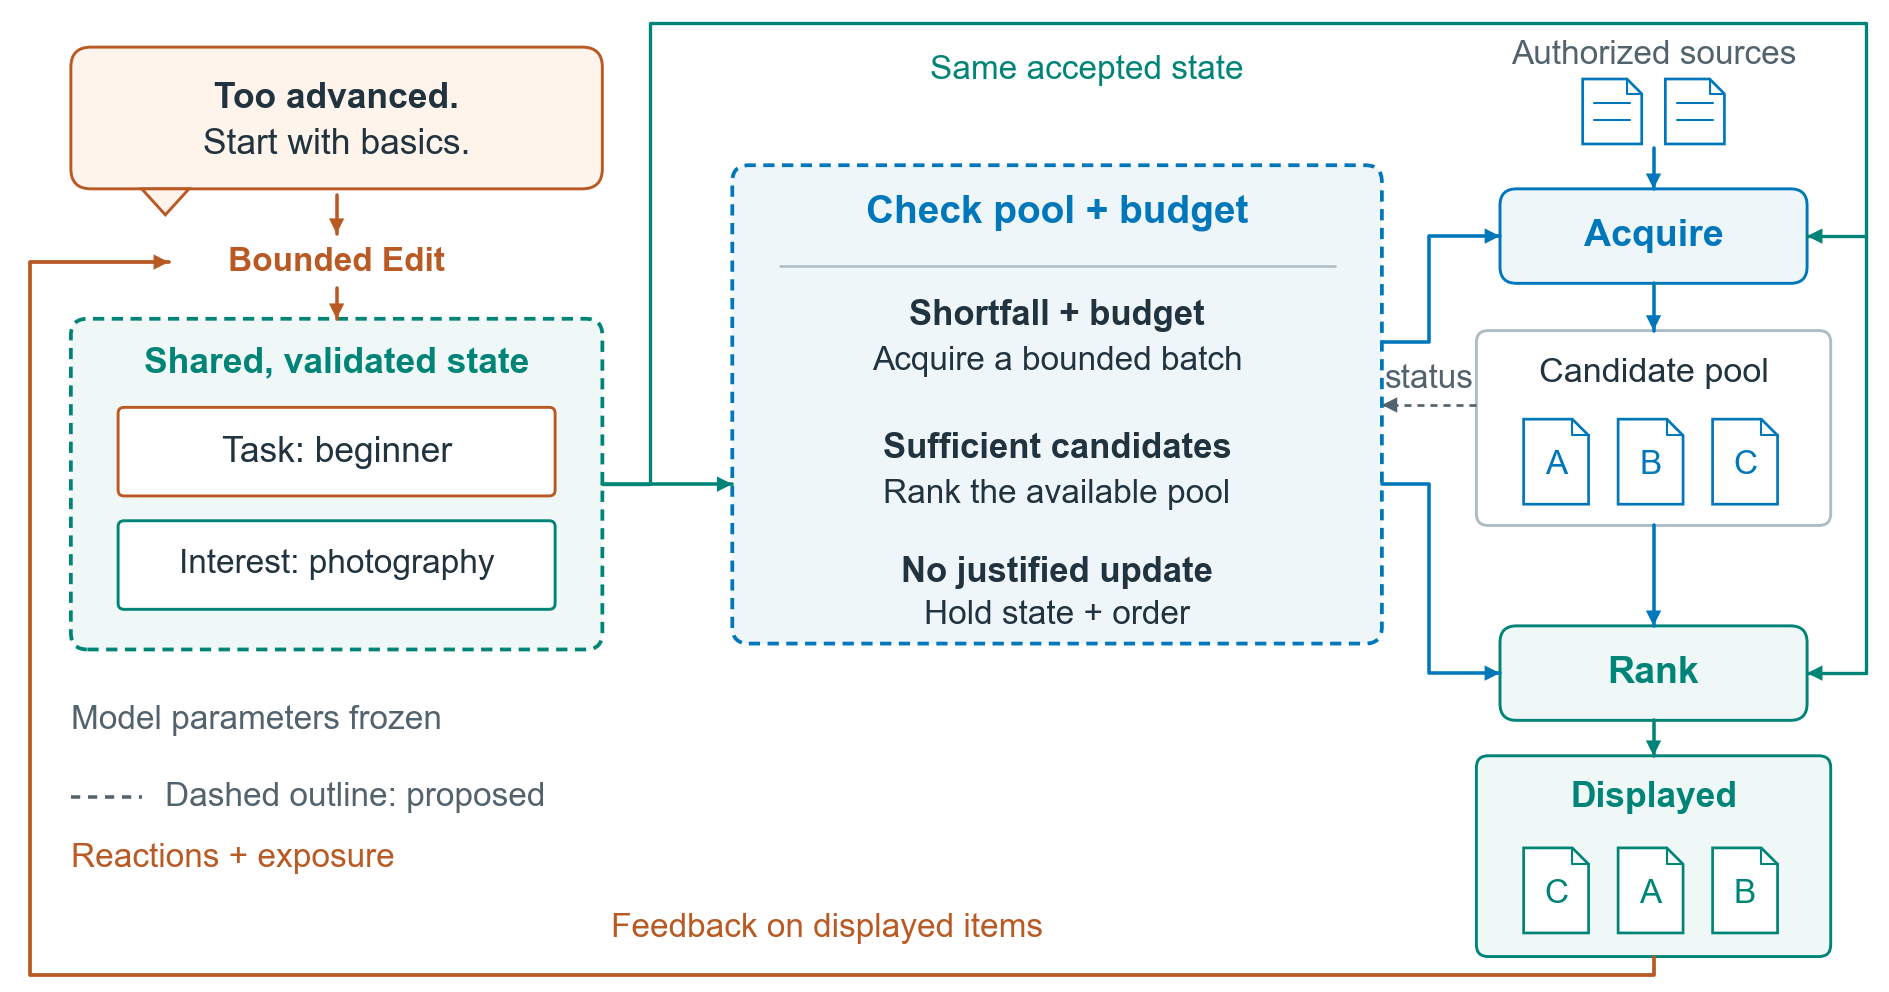
\includegraphics[width=160mm]{../figure-studies/2026-10-21/academic-research/architecture.png}
  \caption{Proposed Waterfall controller. A difficulty correction updates task
  state while preserving a persistent photography interest. Bounded edits produce
  a shared accepted state for acquisition and ranking. The controller checks pool
  sufficiency and budget before acquiring a bounded batch, ranking available
  candidates, or holding. Feedback comes only from displayed items. Model
  parameters remain frozen. Dashed module outlines denote proposed extensions;
  letters are illustrative item identifiers. No measured outcomes are shown.}
  \label{fig:waterfall-academic-study-architecture}
\end{figure*}

\begin{figure*}[t]
  \centering
  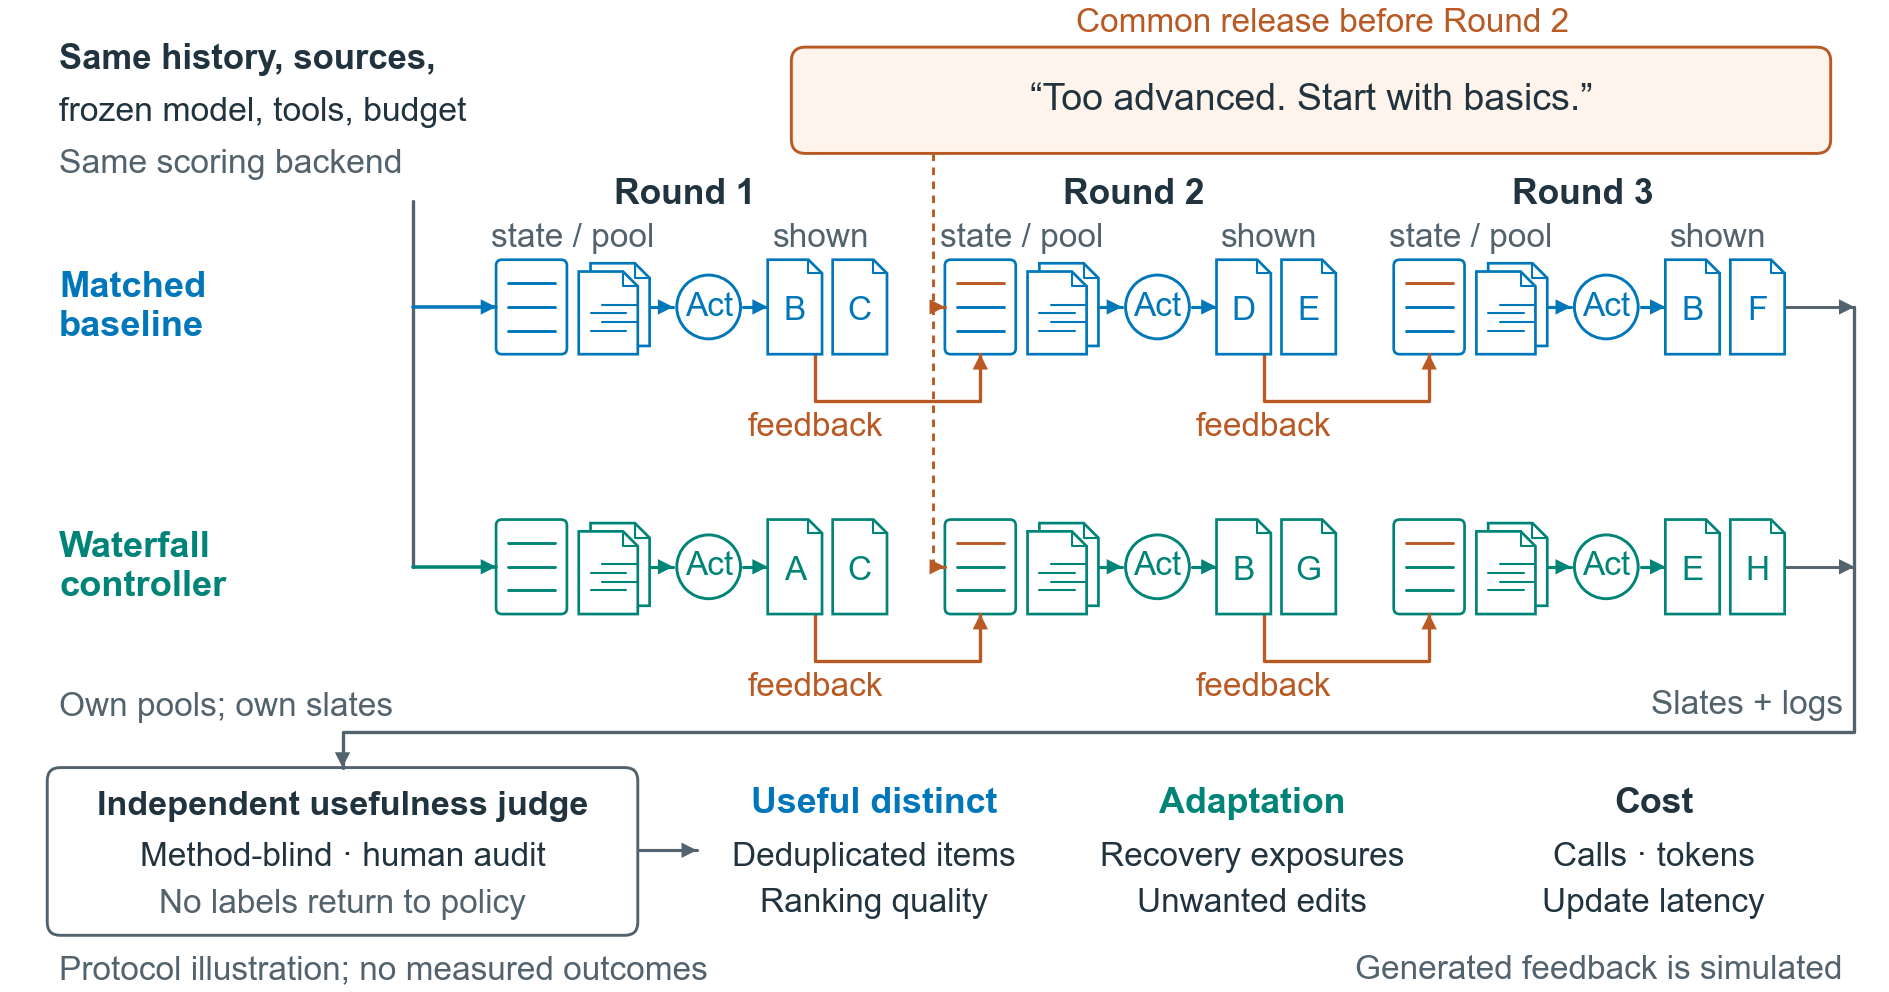
\includegraphics[width=160mm]{../figure-studies/2026-10-21/academic-research/evaluation.png}
  \caption{Planned paired evaluation under matched history, sources, frozen model,
  scoring backend, tools, and budget. Each method maintains its own pool and slate.
  A common correction is released before Round~2; feedback on each method's own
  displayed items updates only its next state. Simulator feedback is synthetic.
  An independent, method-blind usefulness judge is checked by human audit, and its
  labels never return to the policies. Full-trajectory slates and logs support
  usefulness, adaptation, and cost measurements; costs come from execution logs.
  Letters are illustrative identifiers. Three rounds illustrate the protocol,
  not observed results or a fixed final horizon.}
  \label{fig:waterfall-academic-study-evaluation}
\end{figure*}
